%{{{ Formatierung

\documentclass[a4paper,12pt]{article}

\usepackage{physics_notetaking}

%%% dark red
%\definecolor{bg}{RGB}{60,47,47}
%\definecolor{fg}{RGB}{255,244,230}
%%% space grey
%\definecolor{bg}{RGB}{46,52,64}
%\definecolor{fg}{RGB}{216,222,233}
%%% purple
%\definecolor{bg}{RGB}{69,0,128}
%\definecolor{fg}{RGB}{237,237,222}
%\pagecolor{bg}
%\color{fg}

\newcommand{\td}{\,\text{d}}
\newcommand{\RN}[1]{\uppercase\expandafter{\romannumeral#1}}
\newcommand{\zz}{\mathrm{Z\kern-.3em\raise-0.5ex\hbox{Z} }}
\newcommand{\id}{1\kern-.258em1}

\newcommand\inlineeqno{\stepcounter{equation}\ {(\theequation)}}
\newcommand\inlineeqnoa{(\theequation.\text{a})}
\newcommand\inlineeqnob{(\theequation.\text{b})}
\newcommand\inlineeqnoc{(\theequation.\text{c})}

\newcommand\inlineeqnowo{\stepcounter{equation}\ {(\theequation)}}
\newcommand\inlineeqnowoa{\theequation.\text{a}}
\newcommand\inlineeqnowob{\theequation.\text{b}}
\newcommand\inlineeqnowoc{\theequation.\text{c}}

\renewcommand{\refname}{Source}
\renewcommand{\sfdefault}{phv}
%\renewcommand*\contentsname{Contents}

\pagestyle{fancy}

\sloppy

\numberwithin{equation}{section}

%}}}

\begin{document}

%{{{ Titelseite

\title{5 (1.\ Halbtag) $|$ Operationsverstärker}
\author{Angelo Brade, Jonas Wortmann}
\maketitle
\pagenumbering{gobble}

%}}}

\newpage

%{{{ Inhaltsverzeichnis

\fancyhead[L]{\thepage}
\fancyfoot[C]{}
\pagenumbering{arabic}

\tableofcontents

%}}}

\newpage

%{{{

\fancyhead[R]{\leftmark\\\rightmark}

\newpage
\section{Einleitung}

\newpage
\section{Theorie}

\newpage
\section{Voraufgaben}
\subsection{A}
Es gilt die Formel
\begin{align} 
        \dfrac{1}{v}&=\dfrac{1}{v_0}+k&v&=\dfrac{1}{\tfrac{1}{v_0}+k}
.\end{align} 
Für die Werte $k=0.1$, $v_0=10^4$ und $v_0=10^5$ ergibt sich
\begin{align} 
        v_1&\approx 9.990 & v_2&\approx 9.999
.\end{align} 
Mit der Näherung von $v=\tfrac{1}{k}$ ergibt sich
\begin{align} 
        v_\text{Näh}&=10
.\end{align} 
Die Abweichung von $v_1$ und $v_2$ von $v_\text{Näh}$ liegen jeweils bei $0.001\%$ und $0.0001\%$.

\subsection{B}
Es gilt
\begin{align} 
        &&&& U_x &= U_\text{in}-kU_\text{out} &&&& \\
        &&\Leftrightarrow && &= U_\text{in}-kv_0U_x &&&&\nonumber \\
        &&\Leftrightarrow && &= \dfrac{U_\text{in}}{1+v_0k}. &&&&
\end{align} 
Für $k=0.1$, $v_0=10^5$ und $U_\text{in}=\SI{1}{V}$ ist
\begin{align} 
        U_x\approx \SI{0.0001}{V}
.\end{align} 

\subsection{C}
Sei ein Gleichtaktsignal mit $\Delta U_+=\Delta U_-=+\Delta U_\text{in}$.
Dann gilt
\begin{align} 
        &&&& \Delta U_+ &= \Delta U_E+\Delta U_1 & \Delta U_- &= \Delta U_E+\Delta U_1. &&&& 
\end{align} 
Daraus folgt, dass $\Delta U_\text{in}=\Delta U_E+\Delta U_1$.
Die Ausgangsspannung ist
\begin{align} 
        \Delta U_\text{out}=R_C\cdot \Delta I_C
.\end{align} 
An Punkt 1 gilt
\begin{align}
        I_1=2I_E
.\end{align} 
Es ist dann
\begin{align} 
        &&&& \Delta U_\text{in} &= R_E\cdot \Delta I_E+R_1 \cdot 2\Delta I_E = \Delta I_E\left(R_E+2R_1\right)\approx \Delta I_E\cdot 2R_1. &&&& 
\end{align} 
Am Knoten bei $U_\text{out}$ gilt
\begin{align} 
        \Delta I_E=\Delta I_C\Rightarrow \Delta U_\text{out}=R_C\cdot \Delta I_E
.\end{align} 
Die Verstärkung ist dann
\begin{align} 
        v_{CM}=\dfrac{\Delta U_\text{out}}{\Delta U_\text{in}}=\dfrac{R_C}{2R_1}
.\end{align} 
Die Gleichtaktunterdrückung ist
\begin{align} 
        10\log \left(\dfrac{R_E}{R_1}\right)=10\log \left(\dfrac{\SI{1}{\kilo\ohm}}{\SI{100}{\kilo\ohm}}\right)=-\SI{20}{dB}
.\end{align} 

\subsection{D}
Die Frequenzabhängigkeit der Impedanz eines Kondensators ist
\begin{align} 
        Z_1 &= \dfrac{1}{\text{i}\omega C}=\dfrac{1}{\text{i}2\pi fC}\\
        |Z_1| &= \left|\dfrac{1}{\text{i}\omega C}\right| = \dfrac{1}{2\pi fC}
.\end{align} 
Die Verstärkung in Abhängigkeit der Frequenz ist dann
\begin{align} 
        v\left(f\right)=1+\dfrac{Z_2}{|Z_1|}=1+R2\pi fC
.\end{align} 
Die Limits sind
\begin{align} 
        \lim_{f \rightarrow 0}\left[1+R2\pi fC\right] &= 1 & \lim_{f \rightarrow \infty}\left[1+R2\pi fC\right] &= \infty
.\end{align} 
Damit $|Z_1| = R$ ist muss gelten
\begin{align} 
        \dfrac{1}{2\pi fC}=R\Leftrightarrow f=\dfrac{1}{2\pi RC}
.\end{align} 
Für die konkreten Werte $Z_1=R=\SI{100}{\kilo\ohm}$ und $Z_1=C=\SI{100}{\nano F}$ ist die Frequenz
\begin{align} 
        f=\dfrac{1}{2\pi RC}\approx \SI{15.92}{Hz}\Rightarrow v\left(f\right)\approx 2
.\end{align} 
\begin{figure}[h]
        \centering
        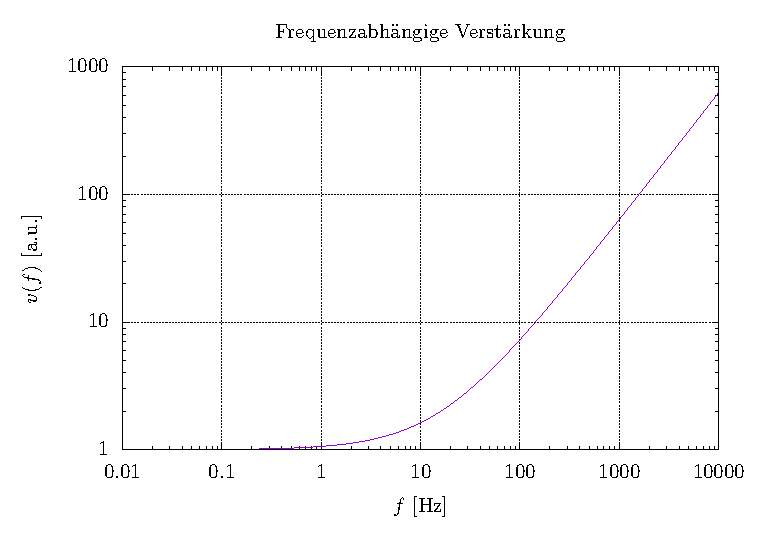
\includegraphics[width=0.7\textwidth]{plot_crop.pdf}
        \caption{Frequenzabhängige Verstärkung eines nicht invertierbaren Verstärkers als Bode--Diagramm}
\end{figure}

\subsection{E}
Sei
\begin{align} 
        v=\dfrac{U_\text{out}}{U_\text{in}}=-\dfrac{Z_2}{Z_1}
.\end{align} 
Das Minuszeichen kommt

\newpage
\section{Auswertung}

\clearpage
\listoffigures
\listoftables
%\bibliographystyle{plain}
%\bibliography{refs}

%}}}

\end{document}
